\section{Graphical User Interface}
\subsection{Game Explorer}

\begin{figure}[h]
	\centering
	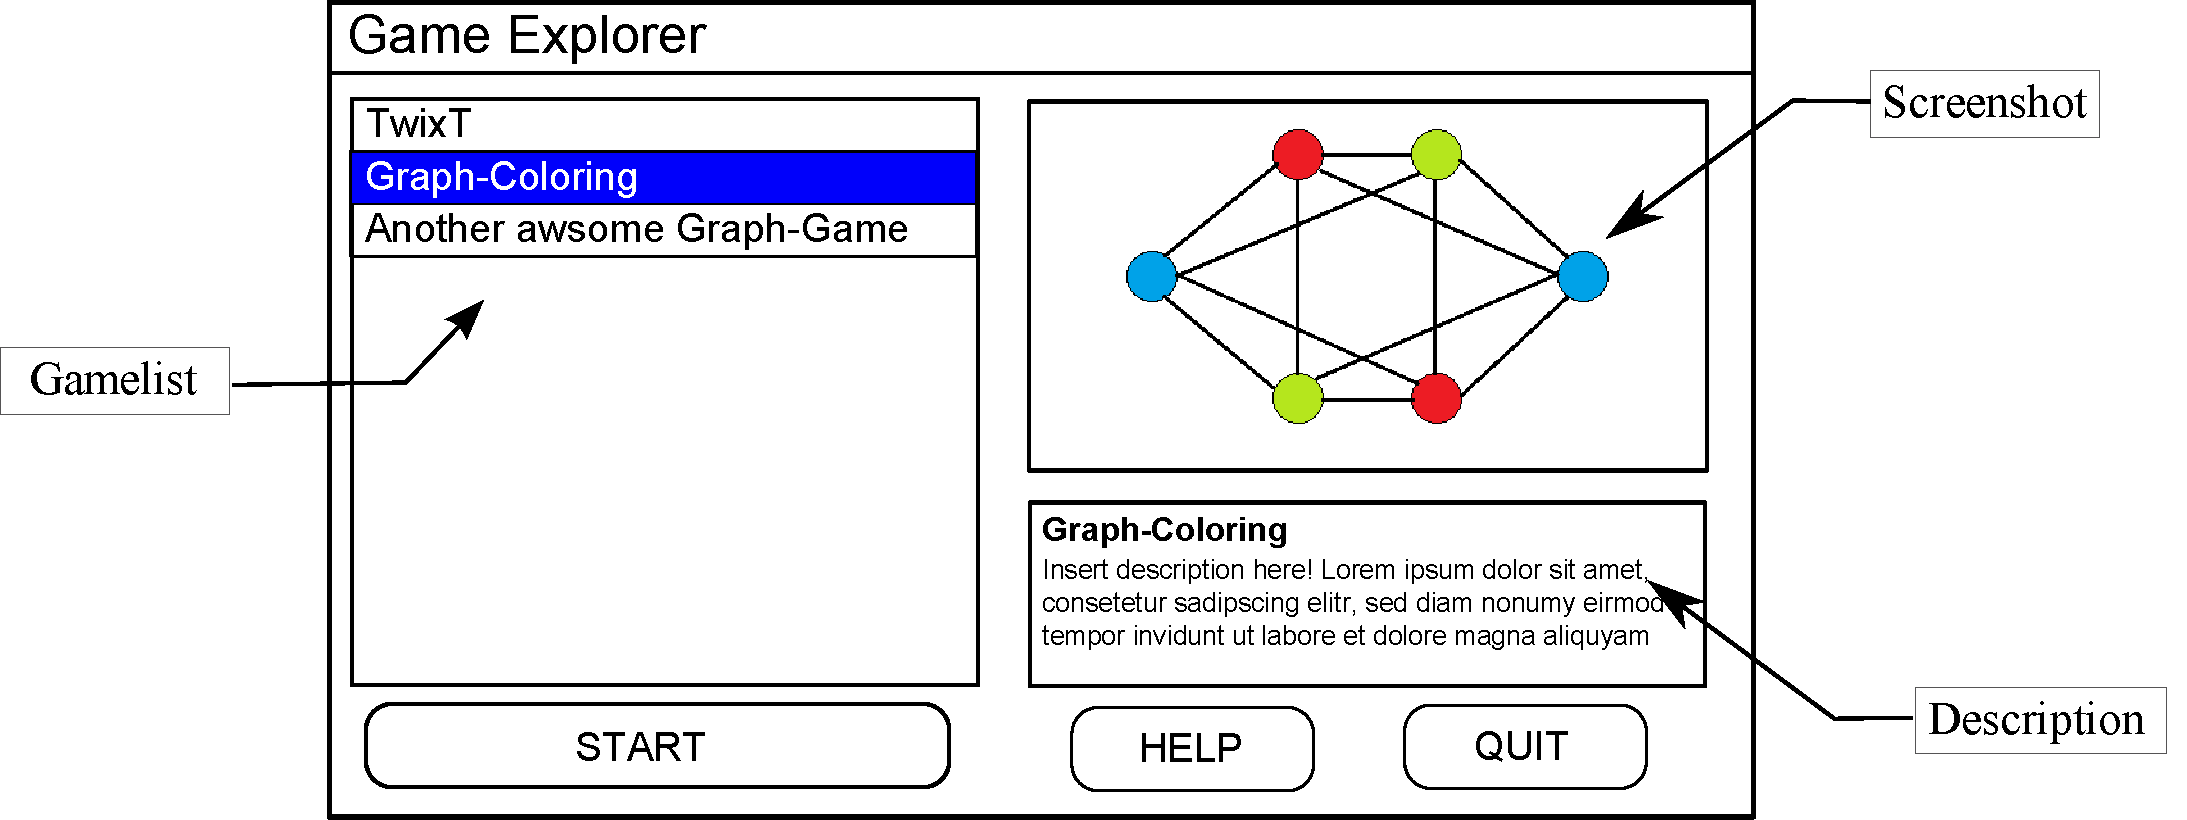
\includegraphics[width=\textwidth]{gui_ge.pdf}
	\caption{Sketch of the Game-Explorer's GUI}
	\label{img:GE_GUI}
\end{figure}

\begin{description}
	\item[Gamelist] Displays a list of available games and is used to select the game the user wants to play.
	\item[Screenshot] Shows a screenshot of the game currently selected.
	\item[Description] Shows a brief description of the game currently selected.
\end{description}

\subsection{Game} \label{REF:GUI_GAME}

\begin{figure}[H]
	\centering
	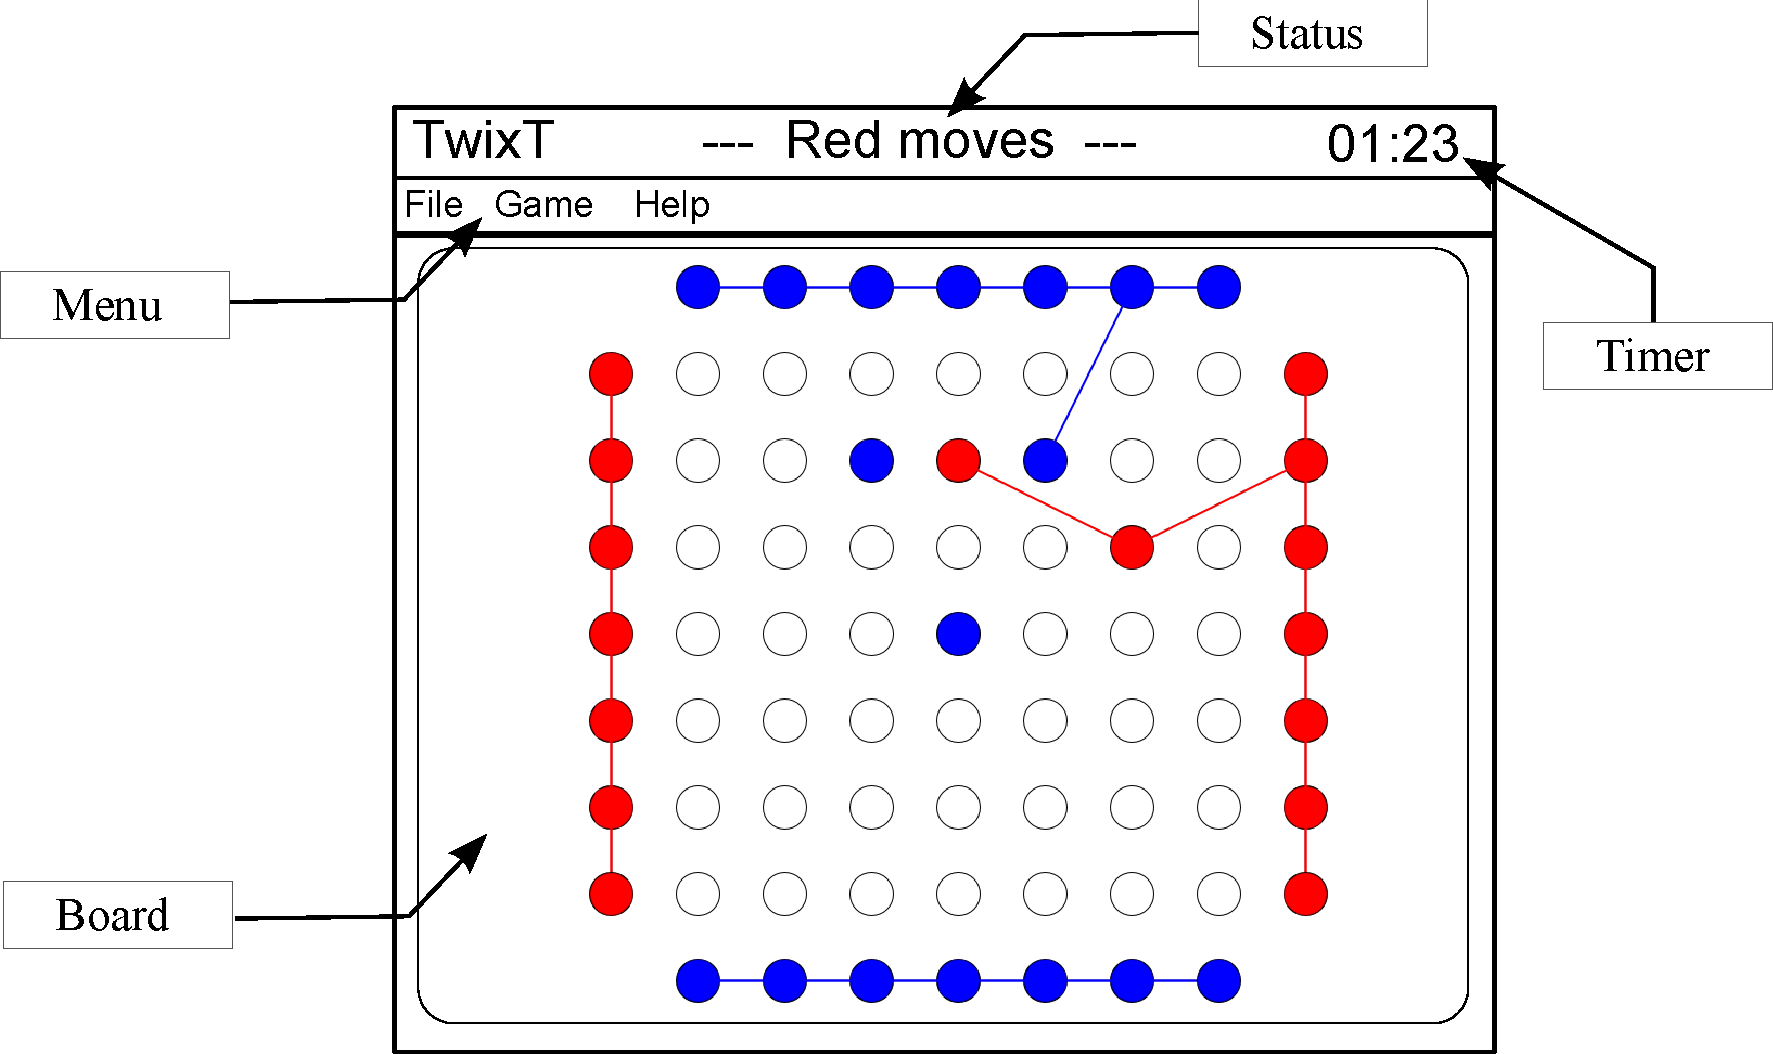
\includegraphics[width=\textwidth]{gui_game.pdf}
	\caption{Sketch of a game's (TwixT) GUI}
	\label{img:GAME_GUI}
\end{figure}

\begin{description}
	\item[Board] Panel where the game's graph is displayed and the main part of the user interaction takes place.
	\item[Status] Gives short information about the game's status.
	\item[Menu] The game's menu.
\end{description}

\subsubsection{File}
\begin{description}
	\item[Restart] Starts the game from beginning.
	\item[Load] Load a previously saved game.
	\item[Save] Saves the state of the current game.
	\item[Exit] Closes the current game.
\end{description}
\subsubsection{Game}
This menu contains game specific options specified by the developer.
\subsubsection{Help}
\begin{description}
	\item[How to play] Shows an explanation of the current game.
	\item[About] Shows information about the current game and the framework,.
\end{description}




